% LTeX: language=de-CH

\section{Methodisches Vorgehen} \label{sec:methodik}

Die vorliegende Arbeit verfolgt ein methodenentwickelndes Ziel: Im Zentrum steht die Konzeption, Umsetzung und Evaluation eines digitalen Erhebungsinstruments zur Analyse des affektiv situativen Wohlbefindens. Dafür wurde eine eigene Smartphone-App (\textit{InterMind}) entwickelt, welche wiederholte, kontextsensitive Befragungen des momentanen Wohlbefindens im Alltag ermöglicht. Methodologisch basiert der Ansatz auf dem Prinzip der \acrfull{esm} sowie deren räumlicher Erweiterung als \acrfull{gema}.

Die entwickelten Instrumente (App und Fragebogen) dienen der Erfassung affektiver Zustände im situativen Kontext, insbesondere mit Blick auf räumliche Umweltfaktoren und soziale Positionierungen. Die so erhobenen Daten werden anschliessend mit Hilfe von \acrfull{maihda} ausgewertet, um intersektionale Effekte auf das subjektive Wohlbefinden modellieren zu können.

Das folgende Kapitel beschreibt zunächst den methodischen Gesamtansatz und begründet die Entscheidung für \acrshort{esm}/\acrshort{gema}. Anschliessend wird die Entwicklung der App dokumentiert, die Durchführung der Datenerhebung beschrieben und die Operationalisierung des Fragebogens erläutert. Abschliessend werden Limitationen des Studiendesigns kritisch reflektiert.


\subsection{Wiederholte Befragung mit \acrshort{esm}, \acrshort{ema} und \acrshort{gema}}

Die systematische Erhebung von momentanen Wohlbefindenszuständen erfordert Methoden, die subjektive Erfahrungen möglichst unmittelbar und kontextspezifisch erfassen. Retrospektive Selbstauskünfte sind hierfür nur begrenzt geeignet, da sie Verzerrungen durch selektive Erinnerung oder nachträgliche Neubewertung unterliegen (\textit{Recall Bias}) \parencite{kahnemanDevelopmentsMeasurementSubjective2006}. Um solche Verzerrungen zu vermeiden, wurde bereits in den 1980er-Jahren die \acrfull{esm} entwickelt. Dieses Verfahren basiert auf der mehrfach wiederholten Erhebung subjektiver Zustände im Alltag – etwa durch zufällig verteilte Signale, die Teilnehmende dazu auffordern, ihre momentane Stimmung, Tätigkeit oder Umgebung zu protokollieren \parencite{csikszentmihalyiValidityReliabilityExperience1987}. Ziel ist es, das Erleben möglichst nah am Zeitpunkt der Erfahrung und im natürlichen Kontext zu erfassen.

Während \acrshort{esm} ursprünglich als psychologisches Messinstrument konzipiert war, wurde der Ansatz in den 1990er-Jahren durch das Konzept der \acrfull{ema} methodologisch erweitert. \acrshort{ema} bezeichnet nicht nur die unmittelbare Erhebung subjektiven Erlebens, sondern schliesst auch physiologische, verhaltensbezogene oder kontextuelle Daten mit ein – etwa über mobile Geräte, Sensorik oder Tagebuchsysteme \parencite{shiffmanEcologicalMomentaryAssessment2008}. Der Begriff „ökologisch“ verweist hierbei nicht auf natürliche Umwelt, sondern auf den Anspruch, Erleben und Verhalten im realweltlichen Lebenskontext zu erfassen – also dort, wo es tatsächlich stattfindet.

Mit der zunehmenden Verbreitung von GPS-fähigen Endgeräten wurde \acrshort{ema} in den 2010er-Jahren durch das Konzept der \acrfull{gema} ergänzt. \acrshort{gema} kombiniert die subjektive Momentaufnahme mit objektiven, räumlich verortbaren Kontextinformationen wie Standort, Wetter, Lärm oder Bebauungsstruktur \parencite{kirchnerSpatiotemporalDeterminantsMental2016}. Im Unterschied zu \acrshort{ema} liegt der Fokus hier auf der systematischen räumlichen Verknüpfung: Subjektive Erfahrungen werden nicht nur als situativ, sondern explizit als räumlich situiert begriffen. Entscheidend ist dabei nicht die Art der Umgebung – also ob es sich etwa um Grünflächen, urbane Plätze oder Transiträume handelt –, sondern die Möglichkeit, affektives Erleben in seiner Beziehung zum jeweils spezifischen räumlich-materiellen Kontext zu analysieren.

Die vorliegende Arbeit folgt diesem methodischen Paradigma. Ziel ist es, situativ affektive Zustände im Raum nicht nur als individuelle, sondern als kontextuell-räumlich bedingte Erfahrungen zu erfassen. Zu diesem Zweck wurde eine eigene Smartphone-Applikation (\textit{InterMind}) entwickelt, die Teilnehmende mehrmals täglich dazu auffordert, eine kurze Selbsteinschätzung ihres momentanen Wohlbefindens und ihrer Umgebungvorzunehmen. Gleichzeitig werden automatisiert Geodaten gespeichert, sodass jede Beobachtung in ihrer konkreten räumlichen Verortung analysiert werden kann. Im Unterschied zu vielen bestehenden GEMA-Studien liegt der Fokus dabei nicht auf spezifischen Umweltmerkmalen wie Vegetationsanteil oder Luftqualität, sondern auf der relationalen Analyse von Raum und subjektivem Erleben.

Die Entscheidung für ein solches Studiendesign bringt gegenüber querschnittbasierten Verfahren mehrere methodische Vorteile mit sich. Erstens reduziert die wiederholte intraindividuelle Erhebung Verzerrungen durch retrospektive Einschätzungen und erlaubt eine präzisere Erfassung situativer Schwankungen. Zweitens ermöglicht sie eine Kontrolle individueller Basisniveaus, was insbesondere für intersektionale Analysen relevant ist, die sowohl zwischen als auch innerhalb von Personen Differenzierungen vornehmen. Drittens erlaubt die Kombination von Echtzeitbefragung und Geodatenanalyse eine kontextsensitive Modellierung der Beziehungen zwischen affektivem Zustand und Umgebung – im Sinne eines relationalen, ökologisch verstandenen Raumbegriffs \parencite{mascherekMeadowsAsphaltRoad2025}.

Für die Erfassung affektiver Zustände wurden numerische Skalen (Slider) eingesetzt als auch Single- und Multiple-Choice-Fragen, die sich in bisherigen Studien als verlässlich und teilnehmendenfreundlich erwiesen haben \parencite{cookeMeasuringWellBeingReview2016}. Die räumliche Verortung erfolgte einerseits über Single- und Multiple-Choice-Fragen, die sich auf die Umgebung des Teilnehmenden beziehen, und andererseits über die Standortdaten der Smartphone-App, wodurch sich subjektive Einschätzungen und objektive Kontextdaten präzise miteinander verknüpfen lassen. Die methodische Grundlage dieser Studie lässt sich somit als eine kritische Anwendung von \acrshort{gema} verstehen, die affektives Wohlbefinden nicht als isolierte Innenwelt, sondern als kontextgebundenes Erleben in Wechselbeziehung von Raum, Situation und sozialer Positionierung begreift.

\subsection{Methodenentwickelnder Charakter und illustrativer Testdurchlauf} \label{sec:methodenentwickelnd}

Diese Arbeit ist als methodenentwickelnde Studie konzipiert. Im Zentrum steht die Entwicklung eines digitalen Erhebungsinstruments, das die situative Erfassung von affektivem Wohlbefinden mit einer intersektionalen Analyse verknüpft. Ziel ist es, einen vollständigen methodischen Workflow zu entwerfen – bestehend aus einem spezifisch konzipierten Fragebogen, einer Smartphone-Applikation zur standortbezogenen Datenerhebung sowie einer vorbereiteten Analysestruktur für für eine intersektionale Modellierung.

Im Unterschied zu klassischen empirischen Studien liegt der Fokus auf der konzeptionellen und technischen Umsetzbarkeit des Ansatzes. Die wenigen im Rahmen der Pilotstudie erhobenen Daten dienen ausschliesslich der Erprobung und exemplarischen Durchführung des methodischen Prozesses – sie erlauben aufgrund der geringen Stichprobengrösse keine  Aussagen über Zusammenhänge zwischen Umgebung, intersektionaler Positionierung und Wohlbefinden.

Die Durchführung einer \acrshort{maihda}-Analyse erfolgt demnach lediglich zu illustrativen Zwecken. Sie diente dazu, die Struktur des Modells zu testen, die Anforderungen an die Datenqualität und -quantität zu reflektieren und das methodische Zusammenspiel von Erhebungsdesign und Analyseansatz zu überprüfen. Auch andere Auswertungsschritte – etwa deskriptive Statistiken oder Visualisierungen – verfolgen keine analytische Zielsetzung im engeren Sinn, sondern dienen der Überprüfung der Funktionsfähigkeit des entwickelten Instruments.

Die methodische Reflexion dieser exemplarischen Anwendung bildet einen zentralen Teil der Arbeit. Sie erlaubt erste Einschätzungen dazu, welche praktischen, technischen oder konzeptionellen Herausforderungen bei der Umsetzung auftreten und wo Anpassungen für künftige Studien notwendig wären. Der wissenschaftliche Mehrwert der Arbeit liegt entsprechend nicht in empirischen Erkenntnissen, sondern in der Bereitstellung und kritischen Diskussion eines erprobten methodischen Zugangs, der für zukünftige Forschungsvorhaben adaptiert und weiterentwickelt werden kann.


\subsection{Vergleich mit bestehenden Erhebungsinstrumenten}

\subsubsection{Tool A: Echtzeiterhebung ohne intersektionale Analyse}

Das \textit{Urban Mind}-Projekt\footnote{Siehe \url{https://www.urbanmind.info/}} stellt ein beispielhaftes Werkzeug dar, um subjektives momentanes Wohlbefinden in städtischen Kontexten mittels Echtzeiterhebungen systematisch zu erfassen und zu analysieren \parencite{bakolisUrbanMindUsing2018}. Es basiert auf einer mobilen Smartphone-App, die mithilfe von Ecological Momentary Assessment (EMA) detaillierte Einblicke in den Zusammenhang zwischen unmittelbaren Umweltfaktoren und mentalem Wohlbefinden ermöglicht.

Zentrales Anliegen des Urban Mind-Tools ist es, die Effekte spezifischer Naturelemente, wie beispielsweise Bäume, Himmel, Wasser oder Vogelgesang, auf das mentale Wohlbefinden in Echtzeit zu untersuchen. Hierfür werden Proband\:innen mehrmals täglich über einen Zeitraum von sieben Tagen aufgefordert, kurze standardisierte Fragen zu ihrer aktuellen Umgebung und ihrem momentanen Wohlbefinden zu beantworten \parencite{bakolisUrbanMindUsing2018}. Die Datenerhebung erfolgt sowohl mittels Selbsteinschätzungen der räumlichen und sozialen Umgebung als auch über Geodaten, welche automatisiert die exakte räumliche Verortung der Teilnehmer\:innen ermöglichen.

\begin{figure}[htbp]
    \centering
    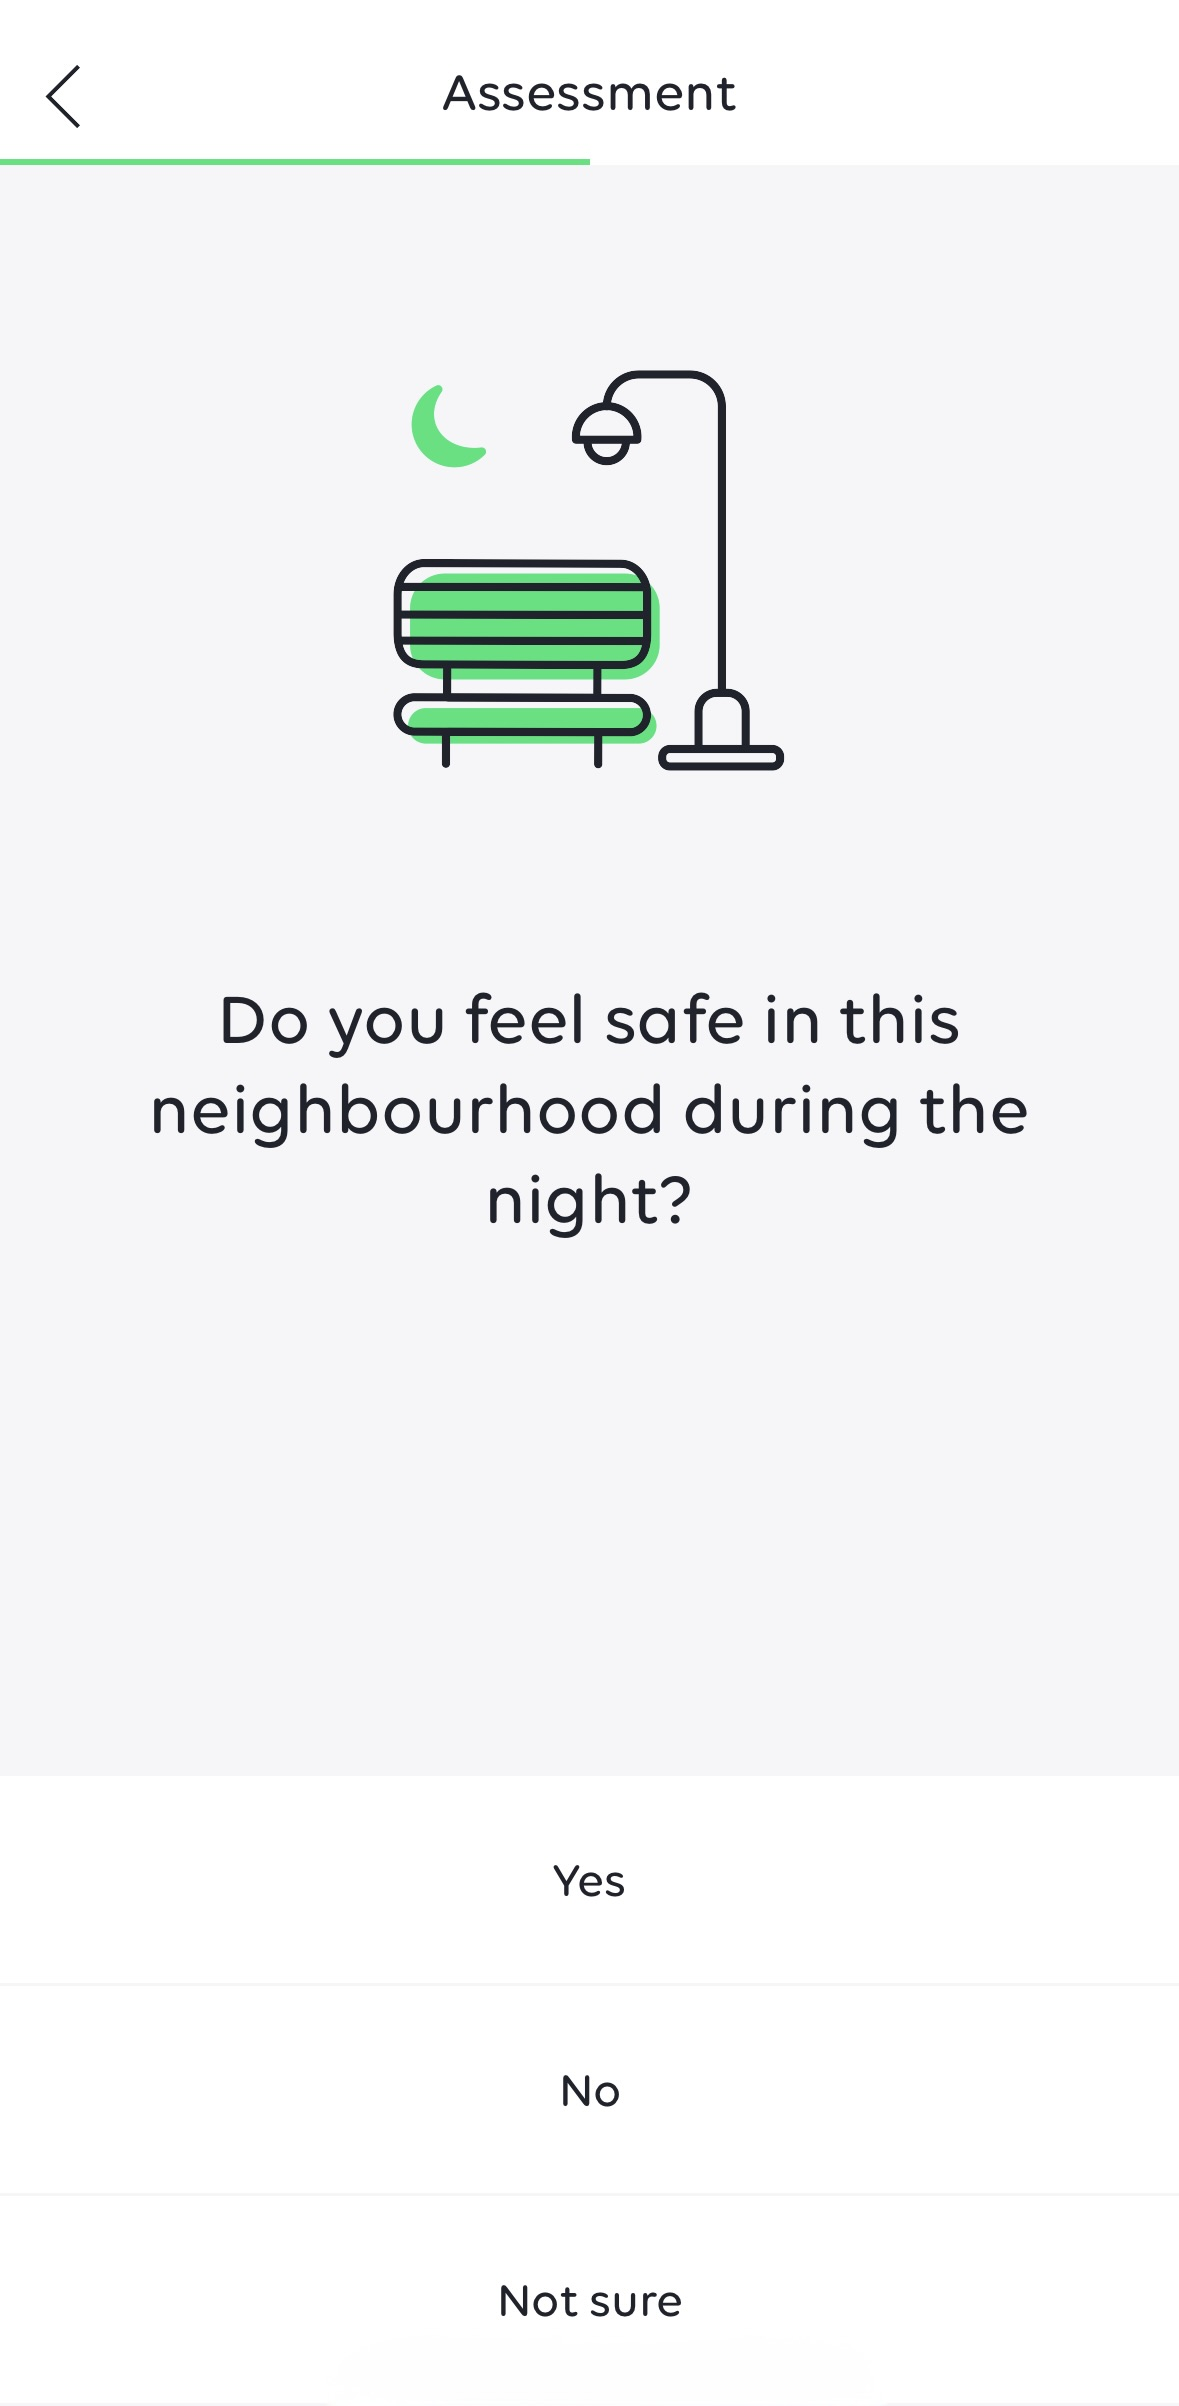
\includegraphics[width=0.5\textwidth]{Arbeit/images/urban_mind01.jpeg}
    \caption{Screenshot einer typischen Frageseite aus der Urban Mind-App}
    \label{fig:urban_mind_screenshot_1}
\end{figure}

Im Gegensatz zu traditionellen querschnittlichen Designs erlaubt das Urban Mind-Tool explizit die Analyse unmittelbarer und zeitverzögerter Effekte (Lag-Effekte). So konnten beispielsweise signifikant positive Effekte von Naturelementen wie Vogelgesang oder dem Sehen von Bäumen auf das momentane Wohlbefinden nachgewiesen werden, welche auch mehrere Stunden nach dem eigentlichen Naturkontakt noch messbar waren \parencite{bakolisUrbanMindUsing2018}. Darüber hinaus betont das Tool die Bedeutung individueller Differenzen und psychologischer Charakteristika, wie beispielsweise Impulsivität, die sich als moderierende Variable herausstellte: Personen mit höherer Impulsivität, welche typischerweise ein erhöhtes Risiko für psychische Erkrankungen aufweisen, profitieren stärker von unmittelbaren Naturerfahrungen.

Hinsichtlich des Designs und der Bedienbarkeit überzeugt die Urban Mind-App durch eine intuitive grafische Gestaltung sowie durch motivierende Elemente wie eine visuelle Übersicht über ausgefüllte und verpasste Fragebögen. Zudem ermöglicht sie Nutzer\:innen, ihre eigenen Daten retrospektiv aufzubereiten, was zu einer angeleiteten Reflexion des eigenen Wohlbefindens beiträgt. Dieses Feature unterstützt insbesondere eine nachhaltige und motivierte Teilnahme über den gesamten Erhebungszeitraum hinweg.

Obwohl Urban Mind zahlreiche methodische und technische Stärken aufweist, berücksichtigt es intersektionale Perspektiven bisher nicht explizit. So sind beispielsweise soziale Kategorien wie Geschlecht, Ethnizität oder sozioökonomischer Status zwar als demografische Variablen erfasst, werden jedoch nicht systematisch in einer intersektionalen Analyse miteinander in Beziehung gesetzt. Theoretisch wäre es möglich, intersektionale Analysen retrospektiv auf Grundlage der erhobenen Daten durchzuführen, eine solche methodische Perspektive wurde jedoch bislang nicht verfolgt.

Die im Rahmen dieser Bachelorarbeit entwickelte App teilt grundlegende methodische Prinzipien mit dem Urban Mind-Tool, wie insbesondere die Nutzung der \gls{ema}-Methode zur Echtzeiterhebung und die Integration räumlicher Kontextinformationen. Im Unterschied zu Urban Mind beinhaltet die entwickelte App jedoch zusätzliche methodische Elemente, wie etwa differenzierte Slider-Fragen, die eine feinere Abstufung subjektiver Empfindungen ermöglichen. Ferner sieht das methodische Konzept dieser Arbeit explizit eine intersektionale Auswertung vor, welche die Urban Mind-Studien in ihrer bisherigen Form nicht integriert haben.

Zusammenfassend lässt sich feststellen, dass Urban Mind in technischer und methodischer Hinsicht ein bewährtes und umfassend validiertes Tool darstellt, dessen methodische Grundprinzipien auch im Rahmen der hier vorliegenden Studie genutzt wurden. Gleichzeitig erweitert die vorliegende Arbeit diesen Ansatz um eine explizit intersektionale Perspektive, welche bisher im Kontext von Echtzeiterhebungen zu räumlichem Wohlbefinden noch unzureichend repräsentiert ist.

Zur Veranschaulichung und besseren Verständlichkeit der methodischen Unterschiede werden im Folgenden ausgewählte Screenshots der Urban Mind-App eingefügt (siehe \Cref{fig:urban_mind_screenshot_1} und Y). Diese zeigen exemplarisch die visuelle Gestaltung der Fragen sowie die ansprechende Übersicht der Teilnehmer\:innen über ihre beantworteten und verpassten Befragungseinheiten, welche als besonders motivierendes Element hervorzuheben sind \parencite{bakolisUrbanMindUsing2018}.

Dieser Vergleich verdeutlicht sowohl methodische Gemeinsamkeiten als auch Unterschiede zwischen den beiden Instrumenten und ermöglicht eine fundierte Einordnung der vorliegenden Studie innerhalb aktueller Ansätze zur Echtzeiterhebung von Wohlbefinden in urbanen Kontexten.


\subsubsection{Tool B: Retrospektive Erhebung und intersektionale Analyse mittels Relief Maps+}

Im Gegensatz zur App „Urban Mind“, die auf eine Echtzeit-Erfassung unmittelbarer Umgebungseinflüsse auf das mentale Wohlbefinden fokussiert, verfolgt das Tool „Relief Maps+“ von Rodó-de-Zárate und Kolleg\*innen einen retrospektiven, explizit intersektionalen Ansatz zur Analyse subjektiver Erfahrungen in unterschiedlichen Räumen und sozialen Kontexten. „Relief Maps+“ ist eine digitale Weiterentwicklung der ursprünglichen „Relief Maps“, die bereits 2014 von Rodó-de-Zárate als empirisches Werkzeug entwickelt wurden, um räumliche, soziale und emotionale Dimensionen intersektionaler Ungleichheiten qualitativ und quantitativ sichtbar zu machen\footnote{Siehe \url{https://reliefmaps.upf.edu/}} \parencite{rodo-de-zarateDevelopingGeographiesIntersectionality2014, luizdesouzaSpiralValidationProcess2025}.

Ziel der „Relief Maps+“ ist es, differenzierte Erfahrungen von Diskriminierung, Unterdrückung, aber auch Privilegien sichtbar zu machen, indem sie drei miteinander verwobene Dimensionen abbilden: die geografische Dimension (konkrete Orte oder räumliche Kontexte), die soziale Dimension (intersektionale Positionierungen wie Gender, Sexualität, Ethnizität oder Alter) und die emotionale Dimension (die subjektiven Gefühle der Teilnehmenden, z. B. Komfort oder Diskomfort). Dadurch werden Machtverhältnisse und deren Auswirkungen auf alltägliche Erfahrungen sowohl räumlich als auch sozial differenziert und emotional nachvollziehbar dargestellt \parencite{rodo-de-zarateIntersectionalitySpatialityEmotions2023}.

Im methodischen Vorgehen erfolgt die Datenerhebung retrospektiv durch ein Online-Formular, in dem die Teilnehmenden ihre subjektiven Erfahrungen in unterschiedlichen sozialen Situationen und an verschiedenen Orten beschreiben. Dabei bewerten sie explizit ihr emotionales Erleben, beispielsweise anhand einer Skala von Komfort zu Diskomfort, und ordnen diese Erfahrungen verschiedenen intersektionalen Positionen (z. B. Geschlecht, Sexualität oder Ethnizität) zu. Daraus resultieren sogenannte „Relief Maps“, die visuell darstellen, an welchen Orten und unter welchen sozialen Bedingungen Diskriminierung oder Privilegierung erlebt wurde \parencite{luizdesouzaSpiralValidationProcess2025, rodo-de-zarateIntersectionalitySpatialityEmotions2023}.

Ein wichtiger Vorteil dieses Ansatzes ist die bewusste und explizite Integration von Reflexivität und Positionalität, da Teilnehmende aufgefordert werden, ihre Erfahrungen in Bezug zu ihren eigenen sozialen Positionierungen kritisch zu reflektieren. „Relief Maps+“ wurde überdies durch ein umfassendes Validierungsverfahren entwickelt, das qualitative, feministische und intersektionale Perspektiven konsequent integrierte. Dabei spielten iterative Feedbackprozesse, Diskussionsgruppen und Pilotstudien eine entscheidende Rolle, um eine ethisch fundierte und theoretisch konsistente Methodik zu gewährleisten \parencite{luizdesouzaSpiralValidationProcess2025}.

Zentraler Aspekt der theoretischen Fundierung von „Relief Maps+“ ist zudem die differenzierte Betrachtung von Emotionen im Zusammenhang mit intersektionalen Ungleichheiten. Gemäss Rodó-de-Zárate fungieren Emotionen als Indikatoren für soziale Positionierungen und Machtverhältnisse, wobei zwischen systematischen Diskomforts, situativen Diskomforts sowie ethischen Diskomforts unterschieden wird. Diese emotionale Perspektive erlaubt es, die komplexen Wechselwirkungen von Orten, sozialen Identitäten und emotionalen Erfahrungen methodisch erfassbar und theoretisch interpretierbar zu machen \parencite{rodo-de-zarateIntersectionalitySpatialityEmotions2023}.

In der Visualisierung der Ergebnisse ermöglichen „Relief Maps+“ die Darstellung von Erfahrungen sowohl individueller als auch gruppenbezogener Art. Die Karten veranschaulichen, wie bestimmte soziale Positionierungen, etwa Geschlecht oder Sexualität, in spezifischen Kontexten systematisch mit Diskriminierung oder Privilegien verbunden sind. Besonders hervorzuheben ist dabei die Fähigkeit des Tools, simultan mehrere Achsen der Unterdrückung und deren räumlich-emotionale Variabilität sichtbar zu machen \parencite{rodo-de-zarateDevelopingGeographiesIntersectionality2014}.

Verglichen mit dem Tool „Urban Mind“ stellt „Relief Maps+“ somit eine tiefer gehende und differenziertere Methodik dar, um intersektionale Dynamiken retrospektiv sichtbar zu machen. Während „Urban Mind“ primär auf unmittelbare Umwelteinflüsse fokussiert und dabei soziale Positionierungen weitgehend unberücksichtigt lässt, setzt „Relief Maps+“ explizit auf eine komplexe intersektionale Perspektive, um systemische und strukturelle Ungleichheiten sichtbar zu machen. Der retrospektive Ansatz erlaubt dabei eine gründliche Reflexion der eigenen Erfahrungen und der sie prägenden gesellschaftlichen Strukturen, bietet allerdings nicht die hohe ökologische Validität und unmittelbare Reaktivität von Echtzeit-Ansätzen wie bei „Urban Mind“.

Für die vorliegende Studie bedeutet dies, dass beide Tools wichtige Anregungen bieten, jedoch unterschiedliche Stärken aufweisen: „Urban Mind“ durch den unmittelbaren, ökologisch validen Zugang zu Alltagserfahrungen, „Relief Maps+“ durch die explizite Integration komplexer intersektionaler Zusammenhänge und deren theoretisch fundierte, räumlich-emotionale Analyse. Beide Perspektiven ergänzen sich methodisch und analytisch, wodurch ein tiefergehendes Verständnis des räumlich situierten, intersektionalen Wohlbefindens erreicht werden kann.


\subsubsection{Einordnung des eigenen Ansatzes}

Die vorliegend entwickelte App greift das Grundprinzip von \emph{Urban Mind} – die mehrfach tägliche Erhebung subjektiver Befindlichkeiten \emph{in situ} – auf und erweitert es in zwei zentralen Punkten:

\begin{enumerate}
    \item \textbf{Methodische Flexibilität.} Neben Single- und Multiple-Choice-Items stehen kontinuierliche Schieberegler sowie optionale Freitextfelder zur Verfügung. Dadurch lassen sich sowohl feingranulare quantitative Einschätzungen als auch kontextspezifische qualitative Informationen erfassen. Die zugrunde liegende React-Native-Codebasis ist modular aufgebaut; neue Fragetypen können mit minimalem Programmieraufwand ergänzt werden.

    \item \textbf{Explizit intersektionale Ausrichtung.} Während \emph{Urban Mind} soziale Kategorien lediglich in der Baseline erfasst, verknüpft der hier gewählte Ansatz zwei Ebenen systematisch: \textit{(i)} detaillierte, einmalig erhobene Soziodemografie (Alter, zugewiesenes und selbstidentifiziertes Geschlecht, sexuelle Orientierung, Behinderung, Einkommen u.\,a.) und \textit{(ii)} situative EMA-Items, die gezielt nach etwaigen Einflüssen eben dieser Merkmale auf das aktuelle Wohlbefinden fragen. Damit wird Intersektionalität nicht nur retrospektiv–korrelativ, sondern \emph{situativ-explizit} operationalisiert.
\end{enumerate}

Die Kombination beider Ebenen erlaubt eine mehrdimensionale Modellierung: Baseline-Merkmale definieren strukturelle Ausgangspositionen, situative Angaben erfassen konkrete Erfahrungen. Durch lineare Mixed-Models oder MAIHDA-Ansätze lassen sich Wechselwirkungen zwischen sozialen Positionen, räumlichen Kontexten und momentanen Befindlichkeiten quantitativ abbilden; Freitextangaben liefern zugleich reichhaltiges Material für eine kontextualisierende, qualitative Vertiefung.

\subsection{Entwicklung der App \textit{InterMind}}

\subsubsection{Ziele und Rahmenbedingungen}

Die zentrale Erhebungslogik der vorliegenden Arbeit basiert auf wiederholten, geolokalisierten Erhebungen zum situativ-affektiven Wohlbefinden der Teilnehmenden. Daraus resultieren spezifische Anforderungen an das digitale Instrument, mit dem diese Daten erfasst werden sollen. Ein geeignetes Erhebungstool muss insbesondere folgende Kriterien erfüllen: Es soll mobil und einfach nutzbar sein, situative Antworten unmittelbar im Alltag der Teilnehmenden ermöglichen, dabei Standortdaten automatisch erfassen und gleichzeitig datenschutzrechtliche sowie technische Hürden für die Nutzer\genderstern innen minimieren. Darüber hinaus war es von Beginn an wichtig, dass das System flexibel und nachhaltig konzipiert ist, um auch über die aktuelle Studie hinaus für zukünftige Forschungsvorhaben eingesetzt werden zu können. Konkret bedeutet dies, dass die Fragenkataloge sowie die Inhalte der App einfach austauschbar und an neue Forschungsfragen oder Zielgruppen anpassbar sein sollten.

Bereits verfügbare Lösungen erfüllten diese Anforderungen nur teilweise oder gar nicht. Kommerzielle Angebote, wie beispielsweise die Forschungsplattform Avicenna\footnote{\href{https://avicennaresearch.com/}{https://avicennaresearch.com/}}, waren aufgrund hoher Lizenzkosten für eine studentische Abschlussarbeit nicht praktikabel. Zudem erlauben solche Dienste in der Regel keine vollständige Kontrolle über die verarbeiteten Daten und bieten nur begrenzte Anpassungsmöglichkeiten hinsichtlich Fragenstruktur und Datenerfassung. Auf der anderen Seite stehen Apps wie Urban Mind\footnote{\href{https://urbanmind.info/}{https://urbanmind.info/}}, die zwar grundsätzlich für \gls{esm}-Erhebungen im Forschungskontext entwickelt wurden, jedoch nicht quelloffen und entsprechend auch nicht eigenständig erweiterbar sind. Gerade im Kontext dieser Studie, bei der sensible Daten zu Wohlbefinden und sozialen Zugehörigkeiten erhoben werden, ist eine transparente und unabhängige Kontrolle der Datenerhebung jedoch von besonderer Bedeutung.

Vor diesem Hintergrund wurde das Ziel formuliert, eine eigene digitale Anwendung zu entwickeln, die bewusst quelloffen und modular gestaltet ist. Diese \gls{opensource}-Architektur sollte es ermöglichen, die gesamte Datenverarbeitung transparent und nachvollziehbar zu gestalten sowie künftige Anpassungen unkompliziert vorzunehmen. Aufgrund der limitierten zeitlichen Ressourcen innerhalb der Bachelorarbeit wurde darüber hinaus darauf geachtet, weit verbreitete Technologien und Frameworks zu wählen, um die Entwicklung möglichst effizient, wartungsarm und für Dritte nachvollziehbar zu halten.

\subsubsection{Konzeptionsphase}
Auf Basis der beschriebenen Anforderungen wurde zunächst ein detaillierter Anforderungskatalog entwickelt, der als zentraler Leitfaden für die weiteren Schritte der App-Entwicklung diente. Dieser Katalog wurde iterativ ergänzt, konkretisiert und während des gesamten Entwicklungsprozesses kontinuierlich an methodische und technische Erkenntnisse angepasst. In Anlehnung an etablierte Konzepte aus der Softwareentwicklung wurde dabei zwischen funktionalen und nicht-funktionalen Anforderungen unterschieden.

Funktionale Anforderungen definieren dabei konkret, \textit{was} die App im praktischen Einsatz leisten muss, und legen somit die notwendigen Funktionen und Abläufe der Anwendung fest. Für diese Studie bedeutete dies insbesondere, dass die App den Teilnehmenden täglich drei zufällig über den Tag verteilte Beantwortungszeiträume von einer Stunde ermittelt und jeweils zum Start dieser Zeiträume \glspl{pushnotification} sendet. Weiter wurde festgelegt, dass bei jeder erfolgten Befragung der aktuelle Standort automatisiert mit erfasst werden soll, sofern die Teilnehmenden dies technisch erlauben. Um die Erhebung flexibel und bedarfsgerecht zu gestalten, wurden zudem verschiedene Fragetypen vorgesehen, darunter Single-Choice, Multiple-Choice, Skalen-basierte Fragen (Slider) sowie Freitextfelder. Schliesslich wurde es als zwingende funktionale Anforderung definiert, dass Teilnehmende jederzeit eigenständig sämtliche gespeicherten Daten löschen können. Die Teilnahme erfolgt dabei vollständig anonym, über eine gerätegebundene, automatisch generierte pseudonyme \gls{uuid}, ohne jegliche Form der Registrierung oder der Eingabe personenbezogener Daten.

Nicht-funktionale Anforderungen legen hingegen fest, \textit{wie} diese Funktionen umgesetzt werden sollen, und beschreiben qualitative Merkmale wie Sicherheit, Benutzerfreundlichkeit oder technische Kompatibilität. In diesem Projekt wurden insbesondere Datenschutz und Datensicherheit als zentrale nicht-funktionale Anforderungen definiert. Sämtliche Datenverarbeitungsprozesse mussten entsprechend den Vorgaben des \acrfull{dsg} und der Europäischen Datenschutzgrundverordnung \acrshort{dsgvo} erfolgen. Weiterhin wurde Mehrsprachigkeit (Deutsch, Englisch und Französisch) als Voraussetzung formuliert, ebenso wie die Möglichkeit einer späteren Erweiterung auf weitere Sprachen. Darüber hinaus sollte die App ursprünglich grundsätzlich offlinefähig sein. Im laufe der Entwicklung wurde diese Anforderung jedoch aufgegeben, da das dazu geführt hätte, dass jede Änderung im Fragenkatalog ein Update der App und anschliessend je nachdem nicht kompatible Versionen der App entstünden. Um Teilnehmenden mit unterschiedlichen Mobilgeräten die Teilnahme möglichst einfach zu machen, war zudem eine plattformübergreifende Kompatibilität für iOS und Android erforderlich. Aus wissenschaftlicher Sicht war schliesslich eine offene, modulare und nachvollziehbare Codebasis wichtig, sodass Anpassungen und Erweiterungen des Systems durch andere Forschende mit minimalem Aufwand möglich bleiben. Dies wurde dadurch erreicht, dass die App als \gls{opensource}-Projekt auf Github\footnote{\href{https://github.com/lbatschelet/intermind}{https://github.com/lbatschelet/intermind}} veröffentlicht wurde.

Die Priorisierung und Auswahl dieser Anforderungen erfolgte unter Berücksichtigung der konkreten Forschungsziele, der vorhandenen Literatur zu mobilen Anwendungen im Bereich \gls{esm} \parencite{chenPerceivedUrbanEnvironment2025, randallDevelopmentTrialMobile2013}, datenschutzrechtlicher Vorgaben sowie praktischer Erfahrungen aus dem eigenen Informatikstudium. Aufgrund des iterativen Vorgehens während der Entwicklung kam es dabei auch später immer wieder zu Anpassungen und Nachjustierungen einzelner Anforderungen – etwa wenn Rückmeldungen aus ersten Testläufen zu veränderten Schwerpunkten führten oder technische Herausforderungen eine Neuausrichtung bestimmter Anforderungen notwendig machten.

\subsubsection{Implementierung}

Für die technische Umsetzung der zuvor definierten Anforderungen wurde als zentrale Entwicklungsumgebung das \gls{framework} \gls{reactnative} in Kombination mit der Entwicklungsplattform \gls{expo} gewählt. Diese Entscheidung ermöglichte es, mit einer einheitlichen Codebasis sowohl iOS- als auch Android-Geräte zu unterstützen, wodurch nicht nur der Entwicklungsaufwand reduziert, sondern auch eine konsistente und vergleichbare Benutzererfahrung auf beiden Plattformen gewährleistet werden konnte. Als serverseitige Infrastruktur wurde \gls{supabase} eingesetzt – ein quelloffenes \gls{backend}-as-a-Service auf Basis einer relationalen \gls{postgresql}-\gls{datenbank}, die Authentifizierung, Datenspeicherung und sichere Datenübertragung integriert bereitstellt.

Beim ersten Start der App generiert das System automatisch eine eindeutige, nicht rückverfolgbare \gls{uuid}, die lokal auf dem Gerät gespeichert wird. Diese \gls{uuid} fungiert als pseudonymisierte Kennung für sämtliche Datenbankoperationen und ersetzt jegliche Form der persönlichen Registrierung. Der eigentliche Fragenkatalog wurde bewusst nicht direkt im Programmcode der App hinterlegt, sondern dynamisch über eine \gls{json}-Konfigurationsdatei geladen, die serverseitig auf der \gls{supabase}-Plattform abgelegt ist. Diese Struktur erlaubt es, den Fragenkatalog jederzeit flexibel und ohne ein zusätzliches App-Update zu ändern oder zu erweitern. Die Kehrseite dieser dynamischen Herangehensweise besteht darin, dass die App zum Laden der Befragungsinhalte auf eine bestehende Internetverbindung angewiesen ist.

Die Zeitpunkte der täglichen Befragungen werden automatisch nach Abschluss des ersten Fragebogens berechnet und anschliessend lokal auf dem Gerät der Teilnehmenden eingeplant. An jedem dieser Slots haben die teilnehmendenden eine Stunde Zeit die Befragung auszufüllen. Dadurch konnten ständige serverseitige Abfragen oder Hintergrundprozesse vermieden werden, was sich positiv auf die Akkulaufzeit und den Datenverbrauch der Geräte auswirkte. Die technische Herausforderung bestand darin, eine zuverlässige und plattformübergreifend kompatible Lösung zur lokalen Planung der \glspl{pushnotification} zu entwickeln, da sich die mobilen Betriebssysteme (iOS und Android) teilweise erheblich in der Handhabung von Hintergrundprozessen unterscheiden.

Das \gls{frontend} der App ist bewusst freundlich und minimalistisch gestaltet, um eine intuitive Nutzung zu gewährleisten und gleichzeitig eine neutrale und unvoreingenommene Wahrnehmung der Fragen sicherzustellen. Die Benutzerführung ist in drei zentrale Bereiche gegliedert: einen Startbildschirm, der den nächstmöglichen Beantwortungszeitraum anzeigt, einen separaten Bereich für den eigentlichen Fragebogen sowie einen Informations- und Einstellungsbildschirm, auf dem umfassende Hinweise zur Befragung und zum Datenschutz hinterlegt sind.

Die Implementierung technischer Anforderungen, wie etwa die Verwaltung von Systemberechtigungen (z. B. Standortfreigabe oder Push-Benachrichtigungen), erfolgte mithilfe von standardisierten Expo-Modulen. Dies vereinfachte viele dieser technischen Herausforderungen erheblich. Hingegen erwies sich die Qualitätssicherung im Laufe des Entwicklungsprozesses als aufwändiger, da keine automatisierte Testsuite implementiert wurde. Fehler wurden daher während der Entwicklung stets manuell identifiziert und behoben. Obwohl dieses Vorgehen im Rahmen der begrenzten zeitlichen Ressourcen pragmatisch war, führte es insgesamt zu einem erhöhten Arbeitsaufwand und erschwerte die systematische und nachhaltige Überprüfung der Softwarequalität.

\subsubsection{Datenschutz und Sicherheit}
Datenschutzaspekte waren von Beginn an zentrale Bestandteile des Entwicklungsprozesses und prägten massgeblich die technische und methodische Umsetzung der App. Dabei wurde konsequent dem Prinzip Privacy by Design gefolgt, welches vorsieht, dass Datenschutzanforderungen bereits bei der Konzeption einer Anwendung berücksichtigt und nicht nachträglich integriert werden. Ziel war es, durch entsprechende technische und organisatorische Massnahmen ein höchstmögliches Mass an Privatsphäre für die Teilnehmenden sicherzustellen sowie gleichzeitig volle Transparenz über die Datenerhebung und -verarbeitung zu gewährleisten.

Die Teilnahme erfolgt ausschliesslich anonymisiert über eine automatisch generierte, gerätegebundene UUID (Universally Unique Identifier). Diese UUID ersetzt vollständig eine Registrierung oder Angabe persönlicher Informationen wie Name, Telefonnummer oder E-Mail-Adresse. Standortdaten werden jeweils ausschliesslich zum Zeitpunkt der Befragung erfasst, eine kontinuierliche Standortverfolgung findet nicht statt. Sämtliche erhobenen Daten – darunter demografische Angaben, situativ-affektives Wohlbefinden, Angaben zur Umgebung und der zum Zeitpunkt der Befragung ermittelte Standort – werden in pseudonymisierter Form auf einem Server in der Schweiz gespeichert.

Als technologische Grundlage für die Datenspeicherung dient die zuvor genannte \gls{supabase}-Plattform mit einer \gls{postgresql}-\gls{datenbank}. Dabei wird eine Zugriffssteuerung auf Zeilenebene \gls{rls} verwendet, um sicherzustellen, dass jedes Endgerät ausschliesslich auf seine eigenen Daten zugreifen kann. Diese technische Massnahme verhindert zuverlässig unberechtigte Zugriffe auf fremde Datensätze. Zudem erfolgt die gesamte Datenübertragung zwischen Endgerät und Server verschlüsselt und über authentifizierte Schnittstellen.

Die Teilnehmenden behalten dabei stets die volle Kontrolle über ihre Daten: Über eine integrierte Funktion innerhalb der App können sämtliche eigenen Datensätze jederzeit selbstständig gelöscht werden. Dies führt zu einer vollständigen und unwiderruflichen Entfernung aller mit der entsprechenden \gls{uuid} verknüpften Daten aus der \gls{datenbank}. Somit liegt die vollständige Kontrolle über die Datenspeicherung zu jedem Zeitpunkt bei den Teilnehmenden selbst.

Alle datenschutzrechtlichen Aspekte, einschliesslich der konkreten Umsetzung der genannten technischen und organisatorischen Massnahmen, sind transparent in einer umfassenden Datenschutzrichtlinie dokumentiert. Diese Datenschutzrichtlinie ist sowohl über die App selbst abrufbar als auch öffentlich über die eigens eingerichtete Website\footnote{\href{https://intermind.ch/privacy-policy.html}{https://intermind.ch/privacy-policy.html}} zugänglich. Darin werden zudem die Rechte der Teilnehmenden gemäss dem \gls{dsg} umfassend dargestellt.

\subsubsection{Test und Iteration}
Zur Sicherstellung der technischen Zuverlässigkeit sowie der Gebrauchstauglichkeit der App wurde im Rahmen dieser Arbeit ein zweistufiger Testprozess durchgeführt. Aufgrund der begrenzten Ressourcen und des Projektumfangs kam dabei keine strukturierte automatisierte Testsuite zum Einsatz. Stattdessen wurde ein pragmatischer Ansatz gewählt, bei dem auftretende Probleme laufend manuell identifiziert und unmittelbar behoben wurden. Obwohl diese Vorgehensweise zu einer insgesamt soliden Funktionalität der Anwendung führte, erwies sich die fehlende automatisierte Qualitätssicherung im Entwicklungsprozess wiederholt als Herausforderung und führte zu einem insgesamt höheren zeitlichen Aufwand bei der Fehlersuche.

In einer ersten Phase fanden fortlaufende technische Funktionstests während der Implementierung statt. Im Fokus dieser Tests standen insbesondere die korrekte Verarbeitung des dynamisch geladenen Fragenkatalogs (\gls{json}-Datei), die fehlerfreie Übertragung von Daten an das \gls{supabase}-\gls{backend}, das Verhalten der App bei unterbrochener oder unzuverlässiger Internetverbindung sowie die plattformübergreifende Zuverlässigkeit der lokalen Planung und Ausführung von \glspl{pushnotification}. Da sich iOS und Android in ihrer Handhabung von Hintergrundprozessen, Benachrichtigungssystemen und Berechtigungsanfragen teilweise stark unterscheiden, wurde der Funktionsumfang regelmässig auf verschiedenen Geräten mit unterschiedlichen Betriebssystemversionen manuell geprüft.

In der zweiten Phase wurde ein interner Pretest mit vier Personen durchgeführt, welche die App über einen Zeitraum von zwei Wochen nutzten. Die Teilnehmenden erhielten hierzu über die offiziellen Beta-Testplattformen (TestFlight für iOS und Google Play Console für Android) Zugang zur Anwendung. Dabei wurden gezielte Aufgaben gestellt, um spezifische technische und inhaltliche Aspekte zu überprüfen sowie allgemeines Feedback zur Benutzerfreundlichkeit und Verständlichkeit der Fragen zu sammeln. Die Rückmeldungen der Testpersonen bezogen sich vor allem auf die Klarheit und Lesbarkeit einzelner Fragen und Texte, auf kleinere Probleme bei der erstmaligen Vergabe von App-Berechtigungen (z. B. Standortzugriff), sowie auf Darstellungsprobleme bestimmter \gls{ui}-Elemente auf verschiedenen Geräten.

Die Ergebnisse aus dieser Testphase führten sowohl zu technischen Anpassungen als auch zu inhaltlichen Änderungen im Fragebogen. Mehrere Fragen wurden sprachlich präzisiert oder gekürzt, einzelne Items wurden ganz gestrichen. Weiterhin wurden Anpassungen an der Benutzeroberfläche vorgenommen, beispielsweise bei Abständen und der Platzierung von Slider-Beschriftungen. Aufgrund der fehlenden automatisierten Tests erforderte jede Änderung erneut eine manuelle Überprüfung der gesamten Funktionalität, was insgesamt erheblichen zusätzlichen Aufwand bedeutete.

Insgesamt ermöglichte der iterative Testprozess jedoch, wesentliche Schwachstellen vor dem Beginn der eigentlichen Datenerhebung zu identifizieren und zu beheben. Obwohl auf eine formalisierte Usability-Evaluation verzichtet wurde, konnten durch diese Vorgehensweise zentrale technische sowie benutzerorientierte Probleme effektiv adressiert werden.

\subsubsection{Veröffentlichung und Distribution}

Um die entwickelte App für die eigentliche Datenerhebung nutzen zu können, wurde eine Veröffentlichung über die offiziellen App-Stores von Apple (iOS) und Google (Android) angestrebt. Beide Plattformen stellen dabei unterschiedliche technische, administrative und finanzielle Anforderungen, die den Veröffentlichungsprozess massgeblich beeinflussten.

Die Veröffentlichung im Apple App Store setzte zunächst den Erwerb einer kostenpflichtigen Entwicklerlizenz voraus, für die eine jährliche Gebühr von CHF 100 zu entrichten war. Nach erfolgreicher Einrichtung dieses Entwicklerkontos wurde die App zur Veröffentlichung eingereicht, allerdings von Apple zunächst nicht für eine finale Veröffentlichung im regulären App Store zugelassen. Als Begründung wurde angegeben, die App weise zu wenig inhaltlichen Mehrwert auf – eine Entscheidung, die aus Sicht der Entwicklung nur schwer nachvollziehbar war. Der Prüfprozess bei Apple ist zum Zeitpunkt des Abschlusses dieser Arbeit noch nicht vollständig abgeschlossen. Dennoch konnte die App über Apples eigene Plattform für öffentliche Beta-Tests („TestFlight“) bereitgestellt werden, sodass Teilnehmende der Studie über einen offiziellen TestFlight-Link Zugang zur App erhielten.

Im Gegensatz dazu verlangte Google für eine Veröffentlichung im Android Play Store keine laufenden Lizenzkosten. Allerdings stellte Google die Bedingung, dass vor einer offenen Betaversion zunächst ein geschlossener Test mit mindestens 20 Personen über einen Zeitraum von zwei Wochen durchgeführt werden musste. Da es innerhalb des zeitlichen Rahmens dieser Bachelorarbeit nicht möglich war, eine ausreichende Anzahl Testpersonen mit Android-Geräten zu rekrutieren, wurde hierfür ein externer Dienstleister in Anspruch genommen, welcher diesen erforderlichen Test für eine Gebühr von CHF 30 durchführte. Nach erfolgreichem Abschluss dieses Tests wurde die App im Play Store als offene Beta veröffentlicht und war somit öffentlich verfügbar.

Darüber hinaus verlangten beide Plattformen, dass eine öffentlich zugängliche Datenschutzrichtlinie zur Verfügung steht. Zu diesem Zweck wurde die Website intermind.ch eingerichtet, auf der neben der vollständigen Datenschutzerklärung auch ergänzende Informationen zum Forschungshintergrund abrufbar sind. Die Kosten hierfür beliefen sich auf einmalig CHF 10 für die Domainregistrierung; Hosting-Kosten entstanden keine zusätzlichen, da auf bereits bestehende Infrastruktur zurückgegriffen wurde.

Durch die Veröffentlichung über offizielle App-Plattformen konnten technische Hürden für die Teilnehmenden minimiert und zugleich plattformspezifische Anforderungen (beispielsweise hinsichtlich Datenschutzrichtlinien und Update-Management) zuverlässig erfüllt werden. Trotz vereinzelter Schwierigkeiten im Freigabeprozess ermöglichte dieses Vorgehen letztlich eine unkomplizierte Distribution und Nutzung der Anwendung im Rahmen dieser Arbeit.

\subsection{Fragebogenstruktur und Operationalisierung}

Der Fragebogen besteht aus zwei zentralen Elementen:

\paragraph{Baseline-Befragung (einmalig):}
Hier wurden grundlegende demografische Variablen (Alter, Geschlecht, sexuelle Orientierung, Behinderung, sozioökonomischer Hintergrund) erhoben, um soziale Positionierungen für spätere intersektionale Analysen verfügbar zu machen. Fragen wurden bewusst offen oder mit freier Spezifikation gestaltet, um Normativität in den Antwortoptionen zu vermeiden und soziale Positionierungen differenziert erfassen zu können.

\paragraph{Situative Befragung (wiederholt):}
Der wiederholt eingesetzte Fragebogen besteht aus kurzen situativen Erhebungen, die mittels EMA durchgeführt wurden. Teilnehmer:innen wurden regelmässig aufgefordert, Fragen zu ihrem momentanen Wohlbefinden (z.\,B. empfundene Sicherheit, Zugehörigkeit, Entspannung) sowie zur aktuellen räumlichen und sozialen Umgebung zu beantworten. Hierbei kamen insbesondere Slider-Fragen zum Einsatz, um eine kontinuierliche Bewertung zu ermöglichen. Ergänzend wurde ein optionales Freitextfeld angeboten, das qualitative Kontextinformationen und subjektive Reflexionen zuliess.

Der Begriff \emph{Operationalisierung} bezeichnet hierbei die konkrete Umsetzung theoretischer Konstrukte in messbare Indikatoren. Wohlbefinden wurde operationalisiert über sieben zentrale Dimensionen (u.\,a. Entspannung, Sicherheit, Zugehörigkeit), die in der Literatur als relevant identifiziert wurden. Räumliche und soziale Kontexte wurden mit Items operationalisiert, die beispielsweise aus der Forschung von Bakolis et al. (2018) übernommen und für die vorliegende Studie adaptiert wurden.

\subsubsection{Ablauf und Durchführung der Datenerhebung}

Die Datenerhebung fand im Rahmen der einführenden Exkursion „Recht auf Stadt“ im ersten Studienjahr des Bachelorstudiengangs Geographie an der Universität Bern im Mai 2025 statt. Die teilnehmenden Studierenden wurden zu Beginn der Exkursion über Zielsetzung und Ablauf informiert und konnten anschliessend freiwillig an der Befragung teilnehmen. Die Nutzung der App wurde über den gesamten Exkursionszeitraum von drei Tagen durchgeführt, wobei die Teilnehmenden via Push-Benachrichtigungen mehrfach täglich aufgefordert wurden, die kurzen situativen Befragungen auszufüllen. Die Baseline-Befragung erfolgte einmalig zu Beginn.

Die Durchführung im Exkursionssetting ermöglichte eine kontrollierte Testung der technischen Funktionalität und eine hohe Compliance bei den Teilnehmenden. Gleichzeitig erlaubte dieses Setting, reale räumliche Kontexte, wie unterschiedliche urbane Umgebungen in Zürich, Basel und Bern, unmittelbar in die Datenerhebung einzubeziehen. Insgesamt zeichneten sich die Daten durch eine hohe räumliche und kontextuelle Varianz aus, die zentrale Grundlage für die späteren intersektionalen Analysen bildete.

Die vollständigen Fragebögen (Baseline- und situative Befragungen) sind als ergänzende Dokumentation digital im GitHub-Repository der App hinterlegt. Dies folgt dem Prinzip offener und transparenter Forschung. Eine detaillierte Fragebogenübersicht kann zusätzlich im Anhang dieser Arbeit eingesehen werden, um die inhaltliche Struktur und die Operationalisierung der theoretischen Konstrukte nachvollziehbar zu machen.

Zusammenfassend stellt die entwickelte App somit ein methodisch differenziertes, technisch flexibles Instrument dar, das sowohl situative Dynamiken als auch intersektionale soziale Strukturen systematisch erfassbar macht. Die enge Verknüpfung mit einem explizit intersektional ausgerichteten Fragebogen ermöglicht es, bestehende methodische Ansätze (Urban Mind, Relief Maps+) gezielt zu erweitern und dabei neue Erkenntnisse zur Beziehung von Raum, Wohlbefinden und sozialer Positionierung zu generieren.


\subsection{Limitationen und Herausforderungen der Datenerhebung}

\subsubsection{Geringe Rücklaufquote und mögliche Ursachen}

\subsubsection{Auswirkungen auf die Datenqualität und Analyse}
